% Figure 4.1: Pipeline Overview

\documentclass[border=5pt,convert={density=300}]{standalone}
\usepackage[utf8]{inputenc}
\usepackage{tikz}
\usetikzlibrary{shapes.geometric,arrows.meta,positioning,calc}

% Define colors
\definecolor{myblue}{RGB}{59,130,246}
\definecolor{mygreen}{RGB}{34,197,94}
\definecolor{myorange}{RGB}{249,115,22}

\begin{document}
\begin{tikzpicture}[
    node distance=0.3cm,
    box/.style={
        rectangle,
        rounded corners=2pt,
        draw=#1!60!black,
        fill=#1!15,
        line width=0.5pt,
        minimum width=1.4cm,
        minimum height=0.45cm,
        align=center,
        font=\fontsize{6}{7}\selectfont
    },
    step/.style={
        rectangle,
        rounded corners=2pt,
        draw=#1!60!black,
        fill=#1!20,
        line width=0.8pt,
        minimum width=2cm,
        minimum height=0.5cm,
        align=center,
        font=\fontsize{6}{7}\selectfont\bfseries
    },
]

% Chapter 3 layer
\node[rectangle, rounded corners=3pt, draw=myblue!50, fill=myblue!5, line width=1pt,
      minimum width=13cm, minimum height=2cm] (CH3) at (0,0) {
    \begin{tabular}{p{1cm}p{11cm}}
        \rotatebox{90}{\fontsize{8}{9}\selectfont\bfseries\color{myblue!70!black}Chapter 3} &
        \begin{tikzpicture}[node distance=0.15cm and 0.2cm]
            \node[box=myblue] (c1) {1. Crawl};
            \node[box=myblue, right=of c1] (c2) {2. Clean};
            \node[box=myblue, right=of c2] (c3) {3. External};
            \node[box=myblue, right=of c3] (c4) {4. Corpus};
            \node[box=myblue, below=of c1] (c5) {5. Weak Label};
            \node[box=myblue, below=of c5] (c6) {6. Annotate};
            \node[box=myblue, below=of c6] (c7) {7. Gold Set};
            \draw[->,>=Stealth] (c1) -- (c2);
            \draw[->,>=Stealth] (c2) -- (c3);
            \draw[->,>=Stealth] (c3) -- (c4);
            \draw[->,>=Stealth] (c4) -- ++(0.2,0) |- (c5);
            \draw[->,>=Stealth] (c5) -- (c6);
            \draw[->,>=Stealth] (c6) -- (c7);
        \end{tikzpicture}
    \end{tabular}
};

% Chapter 4 layer
\node[rectangle, rounded corners=3pt, draw=mygreen!50, fill=mygreen!5, line width=1pt,
      minimum width=13cm, minimum height=1.8cm, below=0.5cm of CH3] (CH4) {
    \begin{tabular}{p{1cm}p{11cm}}
        \rotatebox{90}{\fontsize{8}{9}\selectfont\bfseries\color{mygreen!60!black}Chapter 4} &
        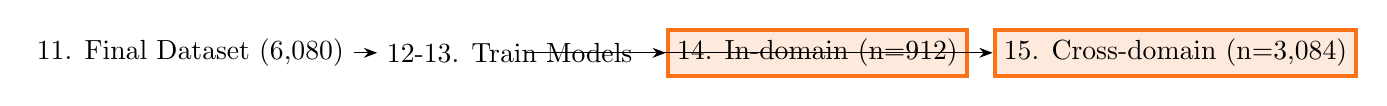
\begin{tikzpicture}[node distance=0.3cm and 0.3cm]
            \node[step=mygreen!60!black] (s11) {11. Final Dataset (6,080)};
            \node[step=mygreen!60!black, right=of s11] (s12) {12-13. Train Models};
            \node[step=myorange, fill=myorange!15, draw=myorange, line width=1.5pt, right=of s12] (s14) {14. In-domain (n=912)};
            \node[step=myorange, fill=myorange!15, draw=myorange, line width=1.5pt, right=of s14] (s15) {15. Cross-domain (n=3,084)};
            \draw[->,>=Stealth] (s11) -- (s12);
            \draw[->,>=Stealth] (s12) -- ++(0.2,0) |- (s14);
            \draw[->,>=Stealth] (s12) -- ++(0.2,0) |- (s15);
        \end{tikzpicture}
    \end{tabular}
};

% Arrow between chapters
\draw[->,>=Stealth, line width=1.5pt, draw=gray!60] (CH3) -- (CH4)
    node[midway, right, font=\tiny, fill=white] {15-step pipeline};

\end{tikzpicture}
\end{document}
